\documentclass[conference]{IEEEtran}
\IEEEoverridecommandlockouts
% The preceding line is only needed to identify funding in the first footnote. If that is unneeded, please comment it out.
\usepackage{cite}
\usepackage{amsmath,amssymb,amsfonts}
\usepackage{algorithmic}
\usepackage{graphicx}
\usepackage{textcomp}
\usepackage{xcolor}
\usepackage{tikz}
\usetikzlibrary{positioning,arrows.meta}
\tikzset{
  arch/.style={draw,rounded corners,align=center,text width=22mm,minimum height=8mm,font=\footnotesize},
  flowstep/.style={draw,rounded corners,align=center,text width=62mm,minimum height=6mm,font=\footnotesize},
  branch/.style={draw,rounded corners,align=center,text width=30mm,minimum height=8mm,font=\footnotesize},
  flowarrow/.style={-{Stealth[length=1.5mm]}}
}

\def\BibTeX{{\rm B\kern-.05em{\sc i\kern-.025em b}\kern-.08em
    T\kern-.1667em\lower.7ex\hbox{E}\kern-.125emX}}
\begin{document}

\title{An IoT Agent for Home and Outing Recommendations Using Indoor Sensing and Weather Forecasts}

\author{\IEEEauthorblockN{KAO CHUN HSUAN, ZHONG YI XIAN, and Xiao Cheng-Yun}
\IEEEauthorblockA{Department of Computer Science and Engineering\\ National Chung Hsing University\\ Taichung, Taiwan}}

\maketitle

\begin{abstract}
Decisions about using indoor appliances, planning outings, and drying laundry depend on information from different places and time periods. This paper proposes an IoT recommendation agent that combines single-room temperature and relative humidity measurements, local weather forecasts, and user feedback. The system associates each recommendation with its supporting measurements or forecasts and their relevant locations and times. A background monitoring process detects sustained environmental changes and requests user confirmation about possible actions, such as operating an appliance or opening a window. The planned evaluation combines chronological event testing, prompt replay, and paired recommendation scenarios to assess event classification, prompting burden, and agreement with the supporting evidence.
\end{abstract}

\begin{IEEEkeywords}
Internet of Things, indoor environmental monitoring, weather forecasts, recommendation agents, user feedback
\end{IEEEkeywords}

\section{Introduction}
Household decisions can depend on both current indoor conditions and expected outdoor conditions. For example, a user deciding where to dry laundry may need the current humidity in a room and the probability of rain at an outdoor location later in the day. Each source describes a different place, time period, and type of observation. A recommendation should make these distinctions clear so that users can judge whether the evidence applies to their situation.

A second challenge is interpreting changes in indoor measurements. A sustained drop in relative humidity can accompany appliance use, ventilation, or changes in temperature. The proposed system treats such changes as candidate events and uses user feedback to associate them with reported actions.

This proposal describes two workflows: an on-demand recommendation workflow that checks the evidence for each response, and a background monitoring workflow that links environmental events to user feedback.

This proposal has three objectives: to link recommendations to their sources, locations, and applicable times; to collect event confirmations while limiting repeated prompts; and to compare classification, prompting, and recommendation methods under shared test conditions.

\section{Related Work}
ReAct provides an example of a language model interleaving reasoning with actions that retrieve external information \cite{yao2023react}. In the proposed system, the agent selects from predefined tools, and the application validates the requested parameters and retrieved records. The UCI Occupancy Detection dataset provides indoor measurements with occupancy labels \cite{uci_occupancy}. In this project, it is considered for checking the preprocessing workflow. Labels for appliance operation will be collected separately through operation logs and user feedback. The CBE Thermal Comfort Tool illustrates the use of multiple inputs in thermal comfort assessment \cite{tartarini2020cbe}. Our single-room prototype will report the limits of recommendations based on temperature and relative humidity measurements.


Prior smart-home research, including CASAS, provides a precedent for collecting residential sensor observations and analyzing daily activities \cite{cook2013casas}. Our target labels describe actions such as operating an appliance or opening a window, so the evaluation requires records collected in the monitored room. Statistical changepoint methods locate changes in a time series \cite{killick2012changepoints}. The proposed prototype uses a sustained-change rule to identify candidate events and links those detections to separately collected operation reports.

Ecological momentary assessment motivates collecting reports close to an event in everyday settings \cite{shiffman2008ema}. Event-triggered prompts ask about possible actions while the context is recent. Because replies can be delayed or uncertain, the system records event onset, prompt time, reply time, and reported operation time separately. Table~\ref{tab:literature} summarizes the implications of the related studies and standards.

\begin{table*}[t]
\caption{Summary of Related Studies and Standards}
\label{tab:literature}
\centering\small
\begin{tabular}{@{}p{.22\textwidth}p{.34\textwidth}p{.39\textwidth}@{}}
\hline
Study or standard & What it provides & Use in this proposal \\
\hline
ReAct \cite{yao2023react} & Language-model reasoning with external tool actions & Route queries to predefined tools and validate retrieved evidence. \\
UCI Occupancy Detection \cite{uci_occupancy} & Indoor readings with occupancy labels & Check preprocessing and collect separate appliance-action labels. \\
CBE Thermal Comfort Tool \cite{tartarini2020cbe} & Assessment using environmental and personal inputs & Explain limits of advice based on room temperature and humidity. \\
CASAS \cite{cook2013casas} & Residential sensing and daily-activity analysis & Motivate room-specific collection and action labeling. \\
Killick et al.\ \cite{killick2012changepoints} & Statistical detection of changes in time series & Contextualize the sustained-change rule. \\
Shiffman et al.\ \cite{shiffman2008ema} & Self-reports close to everyday events & Record prompt, reply, and operation times separately. \\
Roberts et al.\ \cite{roberts2017cv} & Validation of temporally dependent data & Keep events intact and hold out later events for testing. \\
W3C PROV-O \cite{w3c2013provo} & Representation of data and processing provenance & Link recommendations to records and rule versions. \\
OASIS MQTT \cite{oasis2019mqtt} & Publish/subscribe messaging specification & Document the sensor-to-receiver messaging design. \\
\hline
\end{tabular}
\end{table*}

\section{Proposed System}
\subsection{System Architecture}
Figure~\ref{fig:architecture} shows the query and monitoring paths. In the query path, the Web interface captures the question and context. The planner selects permitted tools, the acquisition layer retrieves records, and the analytics engine checks and processes them. The decision module combines these records with versioned domain rules and user preferences. The interface presents the advice with its supporting evidence. In the monitoring path, the same analytics engine processes incoming measurements and creates candidate events. Replies are linked to the corresponding event identifier in SQLite.

\begin{figure*}[t]
\centering
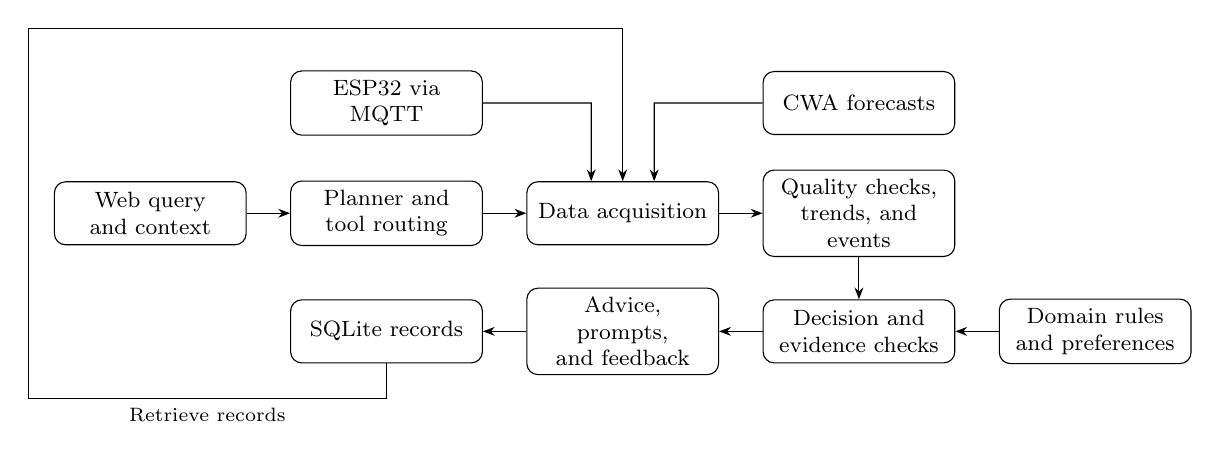
\begin{tikzpicture}
\node[arch] (q) at (0,0) {Web query and context};
\node[arch] (p) at (3,0) {Planner and tool routing};
\node[arch] (d) at (6,0) {Data acquisition};
\node[arch] (a) at (9,0) {Quality checks, trends, and events};
\node[arch] (s) at (3,1.4) {ESP32 via MQTT};
\node[arch] (w) at (9,1.4) {CWA forecasts};
\node[arch] (c) at (9,-1.5) {Decision and evidence checks};
\node[arch] (k) at (12,-1.5) {Domain rules and preferences};
\node[arch] (o) at (6,-1.5) {Advice, prompts, and feedback};
\node[arch] (db) at (3,-1.5) {SQLite records};
\draw[flowarrow] (q)--(p);
\draw[flowarrow] (p)--(d);
\draw[flowarrow] (s.east)--(5.6,1.4)--([xshift=-4mm]d.north);
\draw[flowarrow] (w.west)--(6.4,1.4)--([xshift=4mm]d.north);
\draw[flowarrow] (d)--(a);
\draw[flowarrow] (a)--(c);
\draw[flowarrow] (k)--(c);
\draw[flowarrow] (c)--(o);
\draw[flowarrow] (o)--(db);
\draw[flowarrow] (db.south) -- (3,-2.35) -- node[below,font=\scriptsize]{Retrieve records} (-1.55,-2.35) -- (-1.55,2.35) -- (6,2.35) -- (d.north);
\end{tikzpicture}
\caption{System architecture and data flow. The interaction layer stores user feedback with its associated event identifier.}
\label{fig:architecture}
\end{figure*}

\subsection{Data Acquisition and Alignment}
An ESP32 sensing node will transmit timestamped room temperature and relative humidity (RH) measurements via MQTT. SQLite will store the readings with room identifiers, receive times, and quality flags. Taiwan's Central Weather Administration (CWA) forecasts will be selected by the requested administrative area and validity window \cite{cwa_open_data}. Forecast snapshots will retain retrieval time and the source response. A forecast issue time will be recorded when supplied. The application will check missing values, ordering, continuity, and freshness before analysis.

\subsection{Evidence-Based Recommendations}
As shown in Fig.~\ref{fig:recommendation-workflow}, the workflow retrieves the records required by the user's intent. Outdoor laundry drying requires a forecast for the specified location and time. Comparing indoor and outdoor drying also requires recent room measurements. Python performs numerical checks and applies versioned domain rules. The language model selects from permitted tools, requests clarifications, and explains the recommendation. When an explanation conflicts with verified evidence, the application falls back to a rule-based response template. The response can report source values, locations, applicable times, and any known appliance state. Users operate the appliances themselves.

\begin{figure}[t]
\centering
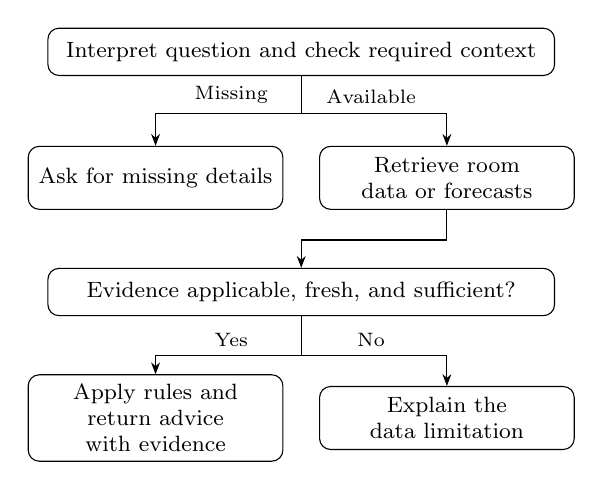
\begin{tikzpicture}
\node[flowstep] (q) at (0,0) {Interpret question and check required context};
\node[branch] (missing) at (-1.85,-1.6) {Ask for missing details};
\node[branch] (fetch) at (1.85,-1.6) {Retrieve room data or forecasts};
\node[flowstep] (check) at (0,-3.05) {Evidence applicable, fresh, and sufficient?};
\node[branch] (yes) at (-1.85,-4.65) {Apply rules and return advice with evidence};
\node[branch] (no) at (1.85,-4.65) {Explain the data limitation};
\draw (q.south)--(0,-.78);
\draw[flowarrow] (0,-.78)-|node[pos=.24,above,font=\scriptsize]{Missing}(missing.north);
\draw[flowarrow] (0,-.78)-|node[pos=.24,above,font=\scriptsize]{Available}(fetch.north);
\draw[flowarrow] (fetch.south)--(1.85,-2.39)-|(check.north);
\draw (check.south)--(0,-3.86);
\draw[flowarrow] (0,-3.86)-|node[pos=.24,above,font=\scriptsize]{Yes}(yes.north);
\draw[flowarrow] (0,-3.86)-|node[pos=.24,above,font=\scriptsize]{No}(no.north);
\end{tikzpicture}
\caption{Evidence-based recommendation workflow. Missing query context is requested before retrieval.}
\label{fig:recommendation-workflow}
\end{figure}

\subsection{Domain Rules and Decision Boundaries}
Table~\ref{tab:domain-rules} distinguishes the evidence required by a rule from the conclusions the system can draw. Each rule applies to a specific intent and checks the relevant time window before producing advice. A room measurement supports advice about the monitored room. An outdoor forecast supports advice for its covered location and interval \cite{cwa_open_data}. When an input is unavailable, the system states which part of the advice remains conditional.

\begin{table}[t]
\caption{Domain rules and decision boundaries}
\label{tab:domain-rules}
\centering\footnotesize
\begin{tabular}{@{}p{.29\columnwidth}p{.33\columnwidth}p{.30\columnwidth}@{}}
\hline
Evidence & Advice or action & Decision boundary \\
\hline
Sustained elevated indoor humidity & Explain the trend and suggest considering dehumidification. & Current device state requires confirmation. \\
Rising temperature with falling relative humidity & Interpret both trends jointly and retain the cause as unknown. & The readings alone do not establish dehumidifier use. \\
Rain possible at the requested location and time & Suggest postponing outdoor drying or preparing for rain when going out. & Advice applies to the forecast location and validity interval. \\
User reports feeling warm indoors & Consider measured conditions and ask about preferences if needed. & Air movement, clothing, and activity are outside the sensing scope. \\
\hline
\end{tabular}
\end{table}

Thermal comfort depends on environmental and personal inputs beyond room temperature and relative humidity \cite{tartarini2020cbe}. In an appliance-use query, the system can explain a sustained humidity increase and offer conditional advice. If the device state is unknown, the response preserves that uncertainty. In a laundry query, the system can compare valid indoor and outdoor evidence, while the decision to use an appliance or move laundry remains with the user.

\subsection{Evidence Records and Worked Example}
The sensing node publishes room measurements through MQTT \cite{oasis2019mqtt}, and a receiver persists them in SQLite. Drawing on the distinction between source entities and processing activities in provenance models \cite{w3c2013provo}, the system links each advice record to the query context, measurement identifiers, forecast snapshots, rule identifier and version, and response status. The measurement time records when the indoor condition was observed. The forecast validity interval records when the prediction applies, and its retrieval timestamp records when the system obtained it.

Consider a user asking whether to move laundry outdoors in the afternoon (Fig.~\ref{fig:laundry-evidence}). The application resolves the drying location and time window before selecting a forecast. A comparison with indoor drying also requires recent valid measurements from the monitored room. If the forecast indicates a chance of rain and the room is humid, the advice may present options such as postponing outdoor drying or choosing a better-ventilated indoor location. Each option is accompanied by the source and applicable time that support it.

If the weather API is unavailable or the available forecast does not cover the requested interval, the response can still report usable indoor measurements and identify the unresolved outdoor conditions. Drying duration also depends on airflow and garment properties, which are outside the measurement scope.

\begin{figure}[t]
\centering
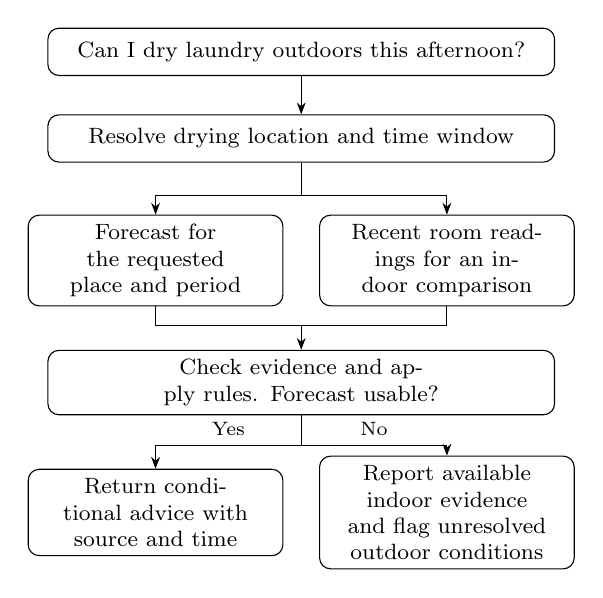
\begin{tikzpicture}
\node[flowstep] (q) at (0,0) {Can I dry laundry outdoors this afternoon?};
\node[flowstep] (ctx) at (0,-1.1) {Resolve drying location and time window};
\node[branch] (fc) at (-1.85,-2.65) {Forecast for the requested place and period};
\node[branch] (rh) at (1.85,-2.65) {Recent room readings for an indoor comparison};
\node[flowstep] (rule) at (0,-4.2) {Check evidence and apply rules. Forecast usable?};
\node[branch] (ok) at (-1.85,-5.85) {Return conditional advice with source and time};
\node[branch] (miss) at (1.85,-5.85) {Report available indoor evidence and flag unresolved outdoor conditions};
\draw[flowarrow] (q)--(ctx);
\draw (ctx.south)--(0,-1.83);
\draw[flowarrow] (0,-1.83)-|(fc.north);
\draw[flowarrow] (0,-1.83)-|(rh.north);
\draw (fc.south)|-(0,-3.47);
\draw (rh.south)|-(0,-3.47);
\draw[flowarrow] (0,-3.47)--(rule.north);
\draw (rule.south)--(0,-5.0);
\draw[flowarrow] (0,-5.0)-|node[pos=.25,above,font=\scriptsize]{Yes}(ok.north);
\draw[flowarrow] (0,-5.0)-|node[pos=.25,above,font=\scriptsize]{No}(miss.north);
\end{tikzpicture}
\caption{Evidence used in a laundry-drying recommendation. The application records forecast validity, indoor observation time when applicable, and the rule version.}
\label{fig:laundry-evidence}
\end{figure}

\subsection{Event Detection and User Feedback}
Figure~\ref{fig:event-feedback-workflow} shows the monitoring workflow. Recent contiguous readings are used to compute smoothed trends and to identify sustained changes. Following a data gap, the application rebuilds the analysis window from valid contiguous measurements. Continuous detections are merged into one event. The prompt policy checks for an unanswered prompt and enforces a minimum interval between prompts. Monitoring continues while the system waits for a reply.

Event onset, prompt time, reply time, and reported operation time are recorded separately. An expired or uncertain reply is recorded as unknown. A late confirmation can be linked to the original event while preserving the earlier record. Operation logs and confirmed replies support event labeling. Confirmed mixed operations are retained, and confirmed periods without actions provide examples of the no-operation class.

\begin{figure}[t]
\centering
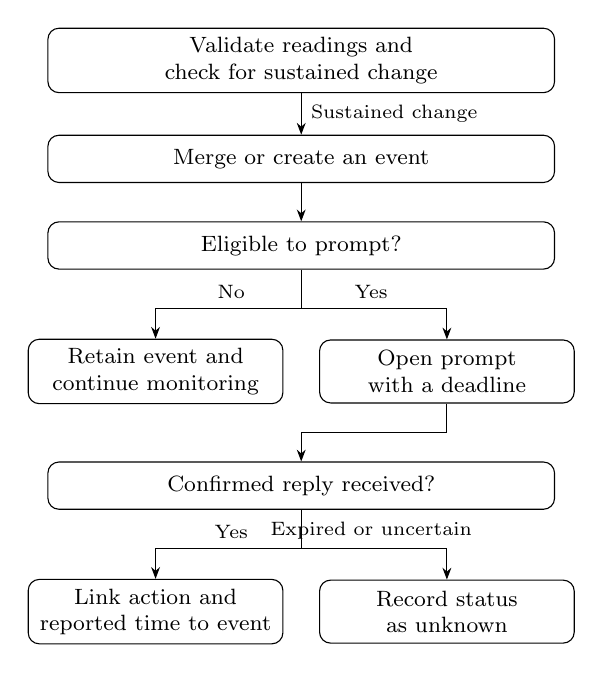
\begin{tikzpicture}
\node[flowstep] (v) at (0,0) {Validate readings and check for sustained change};
\node[flowstep] (e) at (0,-1.25) {Merge or create an event};
\node[flowstep] (p) at (0,-2.35) {Eligible to prompt?};
\node[branch] (defer) at (-1.85,-3.95) {Retain event and continue monitoring};
\node[branch] (ask) at (1.85,-3.95) {Open prompt with a deadline};
\node[flowstep] (r) at (0,-5.4) {Confirmed reply received?};
\node[branch] (y) at (-1.85,-7.0) {Link action and reported time to event};
\node[branch] (u) at (1.85,-7.0) {Record status as unknown};
\draw[flowarrow] (v)--node[right,font=\scriptsize]{Sustained change}(e);
\draw[flowarrow] (e)--(p);
\draw (p.south)--(0,-3.15);
\draw[flowarrow] (0,-3.15)-|node[pos=.24,above,font=\scriptsize]{No}(defer.north);
\draw[flowarrow] (0,-3.15)-|node[pos=.24,above,font=\scriptsize]{Yes}(ask.north);
\draw[flowarrow] (ask.south)--(1.85,-4.72)-|(r.north);
\draw (r.south)--(0,-6.2);
\draw[flowarrow] (0,-6.2)-|node[pos=.24,above,font=\scriptsize]{Yes}(y.north);
\draw[flowarrow] (0,-6.2)-|node[pos=.24,above,font=\scriptsize]{Expired or uncertain}(u.north);
\end{tikzpicture}
\caption{Background monitoring and user feedback. Monitoring continues during pending prompts and when prompting is deferred.}
\label{fig:event-feedback-workflow}
\end{figure}

\subsection{Event Monitoring Protocol}
The event loop handles sensor readings, prompt deadlines, and user replies separately. The monitoring window contains contiguous valid observations. A gap resets that window, so observations collected before a disconnect cannot support a sustained-change decision after recovery. When a change persists, the same event identifier is used for subsequent updates and any prompt tied to that event.

\begin{figure}[t]
\begin{minipage}{\columnwidth}
\small
\begin{algorithmic}[1]
\STATE \textbf{On a new sensor reading:}
\IF{the reading is invalid or follows a data gap}
    \STATE Log the quality issue and reset the analysis window.
\ELSIF{the valid window shows sustained change}
    \STATE Create or update the candidate event.
    \IF{no prompt is pending and the interval has elapsed}
        \STATE Issue a prompt with the event ID and deadline.
    \ENDIF
\ENDIF
\STATE \textbf{On a prompt deadline:}
\IF{no reply has arrived}
    \STATE Record expiry and mark an unconfirmed event unknown.
\ENDIF
\STATE \textbf{On a user reply:}
\STATE Find the event and record reply and reported action times.
\IF{the reply confirms an action or explicitly confirms no action}
    \STATE Save the confirmed label and retain the prompt history.
\ENDIF
\end{algorithmic}
\end{minipage}
\caption{Pseudocode for event monitoring and feedback labeling.}
\label{fig:event-pseudocode}
\end{figure}

Fig.~\ref{fig:event-pseudocode} distinguishes expiry from the event label. For example, a resident may confirm opening a window after the deadline. The prompt history still records that it expired, and the later report can supply the event's confirmed label. An ambiguous reply remains unknown unless another record confirms the action. For binary evaluation, confirmed mixed operations belong to the action class, and their original operation details remain available for inspection.

\subsection{Design Rationale}
Fixed rules provide an interpretable baseline for the first deployment. Their thresholds and persistence settings can be documented and applied to the same held-out events as the decision tree. The learned model may capture interactions between temperature, humidity, and recent trends. Its evaluation depends on the quantity and coverage of confirmed labels. Both approaches will be assessed on the same event partitions, with features limited to information available at decision time.

Event-triggered prompting targets changes that may need clarification, while independent operation logs also record actions that do not trigger the detector. Event merging and a minimum interval reduce opportunities for repeated prompts. Because unanswered prompts and ambiguous replies can change which events obtain labels, the evaluation will report label coverage alongside classification scores. The replay assesses prompt frequency and duplication, and actual interactions provide observed reply rates.

\section{Planned Evaluation}
Approximately two weeks of single-room data collection are planned. The collection will include ordinary periods, independently logged actions, and system-triggered prompts. Table~\ref{tab:evaluation} summarizes the planned comparisons. Thresholds and classifier settings will be selected during development. Complete events will be split chronologically, with later events held out and features restricted to information available at decision time. This respects dependence between nearby observations \cite{roberts2017cv}. All windows derived from an event remain in the same partition. Report confirmed events by class and count unknown events separately from supervised scoring.

\begin{table}[t]
\caption{Planned evaluation comparisons.}
\label{tab:evaluation}
\centering\footnotesize
\begin{tabular}{@{}p{.43\columnwidth}p{.51\columnwidth}@{}}
\hline
Comparison & Planned measures \\
\hline
Fixed rules vs. decision tree & Class counts, precision, recall, macro-F1, confusion matrix \\
Basic prompting vs. event merging and prompt interval & Prompts per hour, repeated-prompt rate, observed reply rate \\
Fixed templates vs. tool-using agent & Tool selection, evidence agreement, appropriate clarification, latency \\
\hline
\end{tabular}
\end{table}

\subsection{Event Classification}
The primary comparison will distinguish recorded actions from explicitly confirmed no-action events. Unknown cases will be counted separately. If there are enough labels, an extension will train the same type of decision tree on independent operation logs alone and on logs augmented with prompted confirmations. Both versions will use the same held-out events to assess the value of the additional labels.

\subsection{Prompt Burden and Recommendation Quality}
The two prompt strategies will be replayed on the same measurement stream to compare prompt frequency and duplication. Prompt frequency is issued prompts divided by monitored hours. The repeated-prompt rate is the fraction of prompted events receiving more than one prompt. The observed reply rate is the fraction of issued prompts with a recorded reply, computed from actual interactions. Fixed templates and the agent will be assessed on the same appliance, outing, and laundry scenarios. Checks will cover location, forecast validity, reported values, known device state, and handling of stale forecasts or API failures.

\subsection{Scenario Construction and Scoring}
Each test case will specify the query, source records available at query time, required evidence fields, and expected behavior. The fixed-template system and tool-using agent will receive the same queries and records. A response passes when it includes the required evidence, matches the source values and time intervals, and avoids unsupported claims about weather or device state. Report both case-level pass rates and field-level error counts. Clarification performance will be scored over cases requiring a question or a statement of data limitations. Measure latency from query submission to availability of the final answer for both systems.

Table~\ref{tab:scenarios} illustrates the acceptance criteria. A stale-forecast case is distinct from a missing-destination case: the former tests forecast validity, while the latter tests whether the system requests essential context before retrieval. In a partial-data case, the user should still receive the source-backed portion of the answer. Each scenario will preserve the input snapshots so that the two approaches can be compared without changes in the live forecast.

\begin{table}[t]
\caption{Example scenarios and acceptance criteria}
\label{tab:scenarios}
\centering\footnotesize
\begin{tabular}{@{}p{.42\columnwidth}p{.52\columnwidth}@{}}
\hline
Test case & Expected behavior \\
\hline
Missing outing destination & Request destination before selecting a forecast. \\
Expired drying forecast & Explain that the forecast fails to cover the requested window. \\
Weather API failure & Report valid indoor evidence and flag outdoor conditions as unresolved. \\
Unknown appliance state & Give conditional advice and keep the state unknown. \\
Indoor and outdoor evidence available & Report the correct room observation time and forecast validity interval. \\
\hline
\end{tabular}
\end{table}

\subsection{Failure-Case Evaluation}
The sensor pipeline will be tested with an isolated spike, a gap followed by valid readings, and a prompt that expires without a reply. The isolated spike should fail the persistence check. After a gap, an event may be considered once the required contiguous window has been re-established. An expired prompt should leave an unconfirmed event labeled unknown. A separate late-reply case will check that an explicit confirmation updates the event record while preserving the earlier expiry. Each check compares the resulting event and prompt records with the expected state transition.

\section{Limitations}
The prototype will observe temperature and relative humidity at one point in one room. Air movement, radiant conditions, clothing, and activity are outside this measurement scope. Reported operation times may be delayed or uncertain, and multiple actions may produce overlapping trends. Township forecasts describe an area and validity window. Their applicability to a specific balcony or outdoor drying site is limited. Sparse labels or class imbalance will limit the interpretation of the classifier comparison.

\section{Conclusion}
This proposal specifies a single-room IoT recommendation agent with source-linked advice and event-linked user feedback. The evaluation will use chronological event splits, paired scenario tests, and prompt replay to examine classification, evidence consistency, and user burden. The results will help define which household decisions the prototype can support with its available measurements and forecast data.

\begin{thebibliography}{10}
\bibitem{yao2023react} S. Yao \emph{et al.}, \emph{ReAct: Synergizing reasoning and acting in language models}, ICLR, 2023.
\bibitem{uci_occupancy} L. Candanedo and V. Feldheim, \emph{Occupancy Detection}, UCI Machine Learning Repository, 2016.
\bibitem{tartarini2020cbe} F. Tartarini, S. Schiavon, T. Cheung, and T. Hoyt, CBE Thermal Comfort Tool: Online tool for thermal comfort calculations and visualizations, \emph{SoftwareX}, vol. 12, Art. no. 100563, 2020.
\bibitem{cwa_open_data} Central Weather Administration, \emph{CWA Open Data API}. [Online]. Available: \texttt{opendata.cwa.gov.tw}
\bibitem{cook2013casas} D. J. Cook, A. S. Crandall, B. L. Thomas, and N. C. Krishnan, CASAS: A Smart Home in a Box, \emph{Computer}, vol. 46, no. 7, 2013, doi: 10.1109/MC.2012.328.
\bibitem{killick2012changepoints} R. Killick, P. Fearnhead, and I. A. Eckley, Optimal detection of changepoints with a linear computational cost, \emph{J. Amer. Stat. Assoc.}, vol. 107, no. 500, pp. 1590--1598, 2012.
\bibitem{shiffman2008ema} S. Shiffman, A. A. Stone, and M. R. Hufford, Ecological momentary assessment, \emph{Annu. Rev. Clin. Psychol.}, vol. 4, pp. 1--32, 2008.
\bibitem{roberts2017cv} D. R. Roberts \emph{et al.}, Cross-validation strategies for data with temporal, spatial, hierarchical, or phylogenetic structure, \emph{Ecography}, vol. 40, pp. 913--929, 2017.
\bibitem{w3c2013provo} W3C, \emph{PROV-O: The PROV Ontology}, W3C Recommendation, Apr. 2013. [Online]. Available: \texttt{www.w3.org/TR/prov-o/}
\bibitem{oasis2019mqtt} OASIS, \emph{MQTT Version 5.0}, OASIS Standard, Mar. 2019.
\end{thebibliography}

\end{document}
